% Created 2023-03-05 Sun 11:31
% Intended LaTeX compiler: pdflatex
\documentclass[11pt]{article}
\usepackage[utf8]{inputenc}
\usepackage[T1]{fontenc}
\usepackage{graphicx}
\usepackage{longtable}
\usepackage{wrapfig}
\usepackage{rotating}
\usepackage[normalem]{ulem}
\usepackage{amsmath}
\usepackage{amssymb}
\usepackage{capt-of}
\usepackage{hyperref}
\usepackage{amsthm}
\author{Yusheng Zhao}
\date{\today}
\title{Homework 4}
\hypersetup{
 pdfauthor={Yusheng Zhao},
 pdftitle={Homework 4},
 pdfkeywords={},
 pdfsubject={},
 pdfcreator={Emacs 28.2 (Org mode 9.6)}, 
 pdflang={English}}
\begin{document}

\maketitle
\tableofcontents


\section{Problem 1}
\label{sec:org1f8acab}
\begin{align}
\psi_{k}(\vec{r}) & = \frac{1}{\sqrt{N}} \sum_{\vec{R}} e^{i\vec{k}\cdot\vec{R}} \phi_{s}(\vec{r} - \vec{R}) \\
& = e^{i\vec{k}\cdot\vec{r}} \frac{1}{\sqrt{N}} \sum_{\vec{R}} e^{i\vec{k}\cdot(\vec{R}- \vec{r})} \phi_{s}(\vec{r} - \vec{R})
\end{align}
Next we only need to show \(\frac{1}{\sqrt{N}} \sum_{\vec{R}}
e^{i\vec{k}\cdot(\vec{R}- \vec{r})} \phi_{s}(\vec{r} - \vec{R})\) is periodic in
lattice vectors. Meaning that if we define \(u(\vec{r}) = \frac{1}{\sqrt{N}}
\sum_{\vec{R}} e^{i\vec{k}\cdot(\vec{R}- \vec{r})} \phi_{s}(\vec{r} -
\vec{R})\), we need to have \(u(\vec{r}) = u(\vec{r}+\vec{R'}\)

\begin{align}
& \frac{1}{\sqrt{N}} \sum_{\vec{R}} e^{i\vec{k}\cdot(\vec{R}- (\vec{r}+\vec{R'}))} \phi_{s}((\vec{r}+\vec{R'}) - \vec{R}) \\
& = \frac{1}{\sqrt{N}} \sum_{\vec{R}} e^{i\vec{k}\cdot((\vec{R}- \vec{R'}) - \vec{r})} \phi_{s}(\vec{r}- (\vec{R} - \vec{R'})) \\
& = \frac{1}{\sqrt{N}} \sum_{\vec{R''}} e^{i\vec{k}\cdot(\vec{R''}- \vec{r})} \phi_{s}(\vec{r}- \vec{R''}) \\
& = \frac{1}{\sqrt{N}} \sum_{\vec{R}} e^{i\vec{k}\cdot(\vec{R}- \vec{r})} \phi_{s}(\vec{r}- \vec{R}) \qed
\end{align}

\section{Problem 2}
\label{sec:orge31d2fd}
\begin{itemize}
\item Let's consider only the nearest neighbor hopping case, and make the strength
\(\gamma = 1 eV\).
\item Let the lattice size be \(a = 0.5\) angstrom.
\item Let's make \(\int \psi^{*}(x)H\psi(x)dx = \epsilon = 4 eV\)
\item \(E(k_{x},k_{y} = \epsilon + 2 * \gamma * (cos(k_{x} * a) + cos(k_{y}*a))\)
\end{itemize}
\begin{verbatim}
using Plots
a = 0.5
ϵ = 4.0
γ = 1.0
kx = -π/0.5:0.01:π/0.5
ky = -π/0.5:0.01:π/0.5
E(kx,ky) = ϵ + 2.0 * γ * cos(kx*a) + 2.0 * γ * cos(ky*a)
# plot(kx,ky,E,st=:surface,camera=(90,90);title="Dispersion Relation",label="E(kx,ky)")
plot(kx,ky,E,st=:surface;title="Dispersion Relation",label="E(kx,ky)")
xlabel!("kx 1/angstrom")
ylabel!("ky 1/angstrom")
zlabel!("Energy (eV)")
\end{verbatim}
\begin{center}
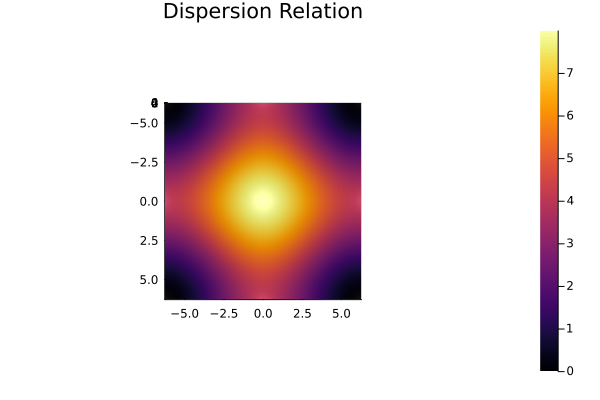
\includegraphics[width=.9\linewidth]{./topview.png}
\end{center}
\begin{center}
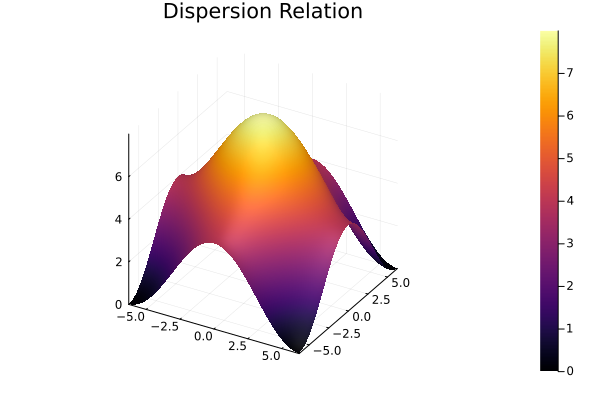
\includegraphics[width=.9\linewidth]{./angle_view.png}
\end{center}
\end{document}